\documentclass[12pt,fleqn]{article}
\setlength{\parindent}{0pt}
\usepackage{graphicx}
\usepackage{cancel}
\usepackage{listings}
\usepackage[latin5]{inputenc}
\setlength{\parskip}{8pt}
\setlength{\parsep}{0pt}
\setlength{\headsep}{0pt}
\setlength{\topskip}{0pt}
\setlength{\topmargin}{0pt}
\setlength{\topsep}{0pt}
\setlength{\partopsep}{0pt}
\setlength{\mathindent}{0cm}

\begin{document}
Dalga Denklemini Turetmek 

Konumuz Kismi Turevsel Denklemler (partial differential equtions -PDE-). Bu
dersin on gerekliliklerinden en onemlisi normal diferansiyel denklemlerdir
(ordinary differential equtions -ODE-), cunku pek cok PDE'yi cozmenin
teknigi onlari bir ODE sistemine indirgemekten geciyor. Yani PDE cozmek
icin ODE cozme tekniklerini de bilmek gerekiyor. Bir diger gerekli bilgi
Lineer Cebir dersi.

Bu dersin ana amaci, bir muhendislik dersi olarak, denklem cozmek, ve pek
cok denklemin cikis noktasi fiziksel problemler. Mesela sicaklik yayilmasi
(heat diffusion), dalga hareketi (wave motion), titresen hucre zari
(vibrating membrane) gibi. Fakat PDE kavrami finansta bile ortaya cikabilen
bir kavram, mesela Black-Sholes denklemlerinde oldugu gibi. 

Yani dersimiz cok teori odakli olmayacak, bazi ispatlardan bahsedecegiz,
ama onun haricinde teori uzerinde fazla durmayacagiz. 

PDE nedir? Ilk once ODE tanimindan baslayalim. 

\[ y = y(x) \]

\[ \frac{dy}{dx} = y \]

Baslangic sartlari 

\[ y(0) = y_0 \]

Cozum 

\[ y = y_0e^x \]

Bu bir ODE cunku sadece bir tane bagimsiz degisken var ($x$), ve bir tane
bagimli degisken var ($y$). 

PDE ise icinde kismi turevleri, ve bir veya {\em birden fazla} bagimsiz
degiskeni barindiran bir denklemdir.

Eger gunes etrafindaki yorungeleri temsil etmek istiyorsaniz gezegenleri
boyutsuz parcaciklar gibi kabul ederek ODE'ler ile temsil etmek yeterli
olabilir, ama diger problemlerde daha fazla bagimsiz degisken gerekecegi
icin ODE yetmez, mesela zaman, cismin 3D uzaydaki boyutlari gibi.

Mesela bir PDE

\[ u = u(x,y) \]

Cogunlukla problem taniminin ilk basinda fonksiyonel iliskiyi hemen
gostermek iyi olur, mesela ustte bagimsiz degiskenler $x,y$, ve $u$ bu iki
degiskene bagimli. Devam edelim PDE soyle olsun

\[ \frac{\partial^3 u}{\partial x^3} + 
cos(y)\frac{\partial u}{\partial y} + 3 = 0
\]

Bir PDE problemine cogunlukla ek olarak sinir kosullari (boundary condition
-BC-) ve baslangic kosullari (initial conditions -IC-) eklemek de gerekir. 

Kismi Turev nedir? 

\[ u = u(x_1, x_2,...,x_n) \]

\[ 
\frac{\partial u}{\partial x_i} = 
\lim_{\Delta x_i \to 0} 
\frac{
u(x_1,..,x_i+\Delta x_i,x_{i+1},...,x_n) - u(x_1,..,x_i,x_{i+1},...,x_n)}
{\Delta x_i}  \]

Yani bir fonksiyonun kismi turevini almak istedigimiz degisken haricinde
tum diger degiskenlerinin sabit tutuldugu bir durum. 

Ornek

\[ u = x_1^2 + x_1sin(x_2) \]

\[ 
\frac{\partial u}{\partial x_1} = 2x_1 + sin(x_2)
 \]

\[ 
\frac{\partial u}{\partial x_2} = x_1 cos(x_2)
 \]

Notasyon

Cogunlukla kismi turevler 3 farkli sekilde gosteriliyor. 

\[ \frac{\partial u}{\partial x} \equiv u_x \equiv \partial_x u \]

Ustte soldaki tanimi gorduk, bazen ortadaki de tercih edilebiliyor, ya da
bazen en sagdaki. 

PDE Derecesi

Bir PDE'nin derecesi, o denklemdeki kismi turevlerin en yuksek dereceli
olanin derecesi neyse o'dur.

Mesela

\[ u_{xxx} + u_y = 5 \]

derecesi 3. Ayni zamanda bu lineer ve homojen olmayan (inhomogeneous) bir
PDE. Bu son iki kavrami birazdan tanimlayacagim. 

Ornek 

\[ (u_{xx})^2 + u_xu_y = u \]

Bu 2. derece. Bu bazi insanlarin kafasini karistiriyor, cunku $u_{xx}$'in
karesi var. Bu ayni zamanda homojen, ve gayri lineer. Bu dersteki cogu PDE
lineer olacak. 

Lineer ve gayri lineerlikten bahsetmisken, sunu ekleyelim. 

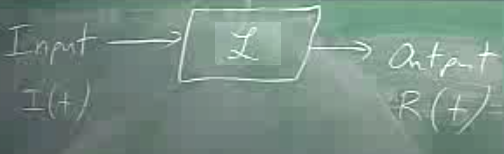
\includegraphics[height=3cm]{1_01.png}

Simdi diyelim ki bir girdi (input) fonksiyonu $I(t)$ bir isleme giriyor
($L$ operatoru) ve cikti (output) olarak $R(t)$ cikiyor. Yani sistem

\[ R = \mathcal{L} \ I \]

Bir lineer sistemde eger girdiyi iki ile carparsaniz, cikti da iki katina
cikar. O zaman kurallar

\begin{enumerate}

   \item $\mathcal{L}(\alpha I) = \alpha \ \mathcal{L}(I)$, ki $\alpha$ bir sabit.

   \item $\mathcal{L}(I_1 + I_2) = \mathcal{L}(I_1) + \mathcal{L}(I_2)$, ki buna ust uste eklenebilme
     (superposition) prensibi deniyor. Bu prensibi bu dersteki cogu PDE'yi
     cozmek icin kullanacagiz. Bir lineer sistem varsa cogu zaman arka
     planda bir yerlerde ust uste eklenebilme prensibi geziniyordur. 

\end{enumerate}

Diyelim ki PDE'nizi soyle yazdiniz

\[\mathcal{L}u = f(\vec{x}) \]

Burada $u$ bagimli degisken, $\vec{x}$ bir vektor, $\vec{x} \in \Re ^n$, ve
bu vektorun icinde birden fazla degisken var, bu degiskenlerin hepsi
bagimsiz.

\[ 
\vec{x} = 
\left(\begin{array}{r}
x_1,\\
.. \\
x_n
\end{array}\right)
 \]

Bu denkleme benzer bir diger denklem lineer cebirdeki $A\vec{x} = \vec{b}$
denklemidir.  PDE sisteminde de cevabini aradigimiz, lineer cebir
sisteminde ``$A$ ile carpilip $b$ sonucunu verecek $\vec{x}$ hangisidir?''
sorusuna benzer bir sekilde ``$\mathcal{L}$ operatoru uygulanip $f(\vec{x})$
sonucunu verecek $u$ hangisidir?'' sorusudur.

Bu analojiden devam etmek gerekirse, belli bir noktada $u$'nun icinde
oldugu ``fonksiyon uzayi'' hakkinda dusunmemiz gerekebilir, $\vec{x}$'in
icinde oldugu $\Re^n$ uzayi gibi. Lineer cebir durumunda operatorun
ozelliklerine bakilir, mesela `` $b$'nin icinde oldugu ve $A$ operatoru
uygulanip hic sonuc alinamayacak uzayin belli kisimlari var
midir?'' gibi sorularla ugrasilabilir, bunlar $A$'nin ``ulasamadigi
yerlerdir'' vs. PDE'deki $\mathcal{L}$ operatoru icin de benzer sorular sorulabilir. 

Yani lineer cebirle pek cok kavram PDE dunyasina benziyor, orada vektor
uzayi var, burada fonksiyon uzayi var. Yani bir analoji olarak bu
benzerligi aklimizda tutmamiz faydali. 

Bir operator su sekilde de olabilir

\[ \mathcal{L} = \mathcal{L} \bigg(
\frac{\partial }{\partial x_1}, \frac{\partial }{\partial x_2},..,
u,..
\bigg)
 \]

Yani operator kismi turevlere ve hatta $u$'nun kendisine de bagimli
olabilir. 

Eger elimizde gayri lineer bir PDE var ise, basimiz dertte demektir. Boyle
bir sistemi cozmek icin cogunlukla sayisal cozumlere basvurmak
gerekir. Eger lineer ise cozumde bayagi ilerlemek mumkundur. 

Lineerlik

Bir operator ve onun tanimladigi bir ust uste eklenebilme durumu dusunelim

\[ \mathcal{L} = \mathcal{L}(\alpha_1 u_1 + \alpha_2 u_2) = 
\alpha_1 \mathcal{L}u_1 + \alpha_2 \mathcal{L}u_2 \]

ki $\alpha_1,\alpha_2$ birer tekil sayidir (scalar), ya reel, ya da kompleks. 

Ornek

Birazdan bakacagimiz denklem dalga denklemi. Orada

\[ u_{tt} - c^2u_x = 0 \]

Bu denklemi

\[ \mathcal{L}u = 0 \]

seklinde yazabiliriz ki $\mathcal{L}$ soyle tanimli olacaktir

\[ \mathcal{L} = \frac{\partial^2}{\partial t^2} - 
c^2 \frac{\partial ^2}{\partial x^2 = 0}\]

$c$ bir sabittir. 

Simdi diyelim ki su denklemi cozmemiz lazim

\[\mathcal{L} u = f \]

ki

\[ \mathcal{L}: V \to V \]

Yani, $\mathcal{L}$ bir vektor uzayini bir digerine eslemekte (map), ve yine diyelim
ki bu uzaylar birer Hilbert Uzayi (bunun anlamina simdi bilmemiz
gerekmiyor, ileride bu konuya donecegiz, bu kelimeyi soyle bir ortaya atmak
istedim). 

Yani sordugumuz Hilbert Uzayi $V$'de bir $f$'e esleyecek bir $u$ fonksiyonu
olup olmadigi. Bu arada tipik bir Hilbert Uzayi mesela kare alip bir sinir
bolgesinde (boundary domain) entegre edince elde edilen sonlu (finite) bir
sonuclarin olusturdugu uzay. Yani ``derli toplu'' fonksiyonlar bir anlamda,
absurt sonuclar vermeyen turden, sonsuzluga dogru patlayip giden turden
olanlari degil. 

Faraziyeye devam edelim, diyelim ki $V$ icinde bir baz (basis) var. Baz
nedir? Lineer cebirden hatirlayalim, mesela uc boyutlu Oklidsel (Euclidian)
uzayi $\Re^3$. 

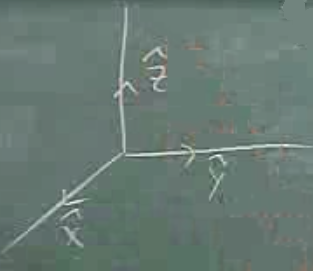
\includegraphics[height=4cm]{1_02.png}

\[ 
\vec{x} = 
\left[\begin{array}{r}
1 \\ 0 \\ 0
\end{array}\right]
 \]

\[ 
\vec{y} = 
\left[\begin{array}{r}
0 \\ 1 \\ 0
\end{array}\right]
 \]

\[ 
\vec{z} = 
\left[\begin{array}{r}
0 \\ 0 \\ 1
\end{array}\right]
 \]

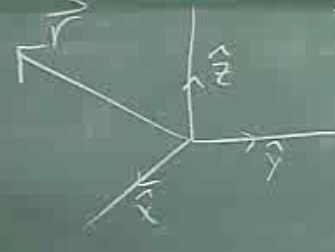
\includegraphics[height=4cm]{1_03.png}

Bu uzaydaki herhangi bir vektor $\vec{r}$ ustteki uc baz vektoru
kullanilarak parcalarina ayirilabilir, ya da, onlarin bir lineer
kombinasyonu olarak gosterilebilir. Mesela

\[ \vec{r} = x\vec{x} +  y\vec{y} +  z\vec{z} \]

Bu uc vektorun bu uzay icin bir ``baz olusturdugu'' soylenebilir, cunku bu
uzaydaki her vektor bu uc vektorun bir kombinasyonu olarak temsil
edilebilir. Dikkat edelim, iki baz vektor yeterli olmazdi, dort taneye
gerek yok. Tami tamina uc tane vektor bu uzayin bazini olusturuyor. 

Bu sonlu (finite) miktarda bir uzay, herhangi bir vektoru tanimlamak icin
sonlu miktarda baz vektoru yeterli. Sonsuz boyutlu bir uzay da olabilirdi,
o zaman herhangi bir fonksiyonu tanimlamak icin sonsuz tane baz vektoru
gerekirdi. Mesela Fourier Serilerini dusunelim

\[ u = \sum_{i=1}^{\infty} \alpha_i \phi_i(x) \]

ki baz fonksiyonlar $\bigg\{ \phi_i(x)  \bigg\}_{i=1}^\infty$.

Bu fonksiyonlarin her biri trigonometrik fonksiyonlar olabilir (cos, sin)
gibi, o zaman seri Fourier Serisi olur. Her halukarda, yukaridaki tanimla
diyoruz ki belli (unique) $\alpha$ degerleri var ki, o degerleri zaten
onceden bilinen baz fonksiyonlari ile carpip toplayarak $u$'yu
olusturabiliyoruz.

Eger lineer operatorumuzu hatirlarsak

\[ \mathcal{L} = \mathcal{L}(\alpha_1 u_1 + \alpha_2 u_2) = 
\alpha_1 Lu_1 + \alpha_2 Lu_2 \]

Bu operator herhangi iki katsayiyi kullaniyordu, fakat iki ustteki sonsuz
tane toplami da icerecek sekilde genisletilebilir, ve baz kavrami ile ust
uste eklenebilme kavraminin arasindaki alakayi gosterir. 

Diyelim ki $\mathcal{L}$'nin her baz vektorunu nasil esledigini biliyoruz, 

\[ \mathcal{L} \phi_i = -\lambda_i \phi_i \]

Ustteki ifade $\phi$'in $L$'in ozfonksiyonu oldugunu soyluyor ayni
zamanda. Eger alttaki acilimi yaparsak, ki bunu yapabiliriz cunku
$\phi$'ler bazdirlar, 

\[ \mathcal{L}u = \mathcal{L} \bigg( \sum_i \alpha_i \phi_i(x) \bigg) =
\sum_i \alpha_i \bigg( \mathcal{L} \phi_i \bigg)
 \]

\[ = -\sum_i \alpha_i \lambda_i \phi_i  \]

Bir operatorun herhangi bir baz uzerinde nasil islem yaptigini anladigimiz
anda, o zaman $\mathcal{L}$'in herhangi bir $u$ fonksiyonu uzerinde ne etki yaptigini
bilebiliriz. Diger bir deyisle bir uzayda sonsuz tane fonksiyon olabilir,
ama biz operatorumuzun bazlara nasil etki ettigini biliyorsak, o bazlarla
olusturulan tum fonksiyonlara nasil etki ettigini de biliyoruz demektir. 

Tekrar belirtelim, bu sadece $\mathcal{L}$ lineer bir operator oldugu zaman mumkun. 

Ornek

Klasik Burger denklemi

\[ u_t + u u_x = v u_{xx} \]

Denklemi 

\[ \mathcal{L}u = 0 \]

olarak yazabiliriz, ki 

\[ \mathcal{L} = \frac{\partial }{\partial t} + 
u \frac{\partial }{\partial x} - v\frac{\partial ^2}{\partial x^2}
\]

Bu gayri lineer

Ornek

\[ u_{xx} + u_{yy} + sin(u) \]

\[ \mathcal{L} u = 0 \]

\[ \mathcal{L} = \partial_{xx} + \partial_{yy} + sin(\cdot) \]

Usttteki ilginc bir durum sinus fonksiyonun da ici bos halde, operator
olarak kullanilmis olmasi. Operator taniminda bazen boyle nokta konuldugu
oluyor, ki neyin uzerinde operasyon yapildigi anlasilsin diye, mesela
ustteki soyle de gosteriliyor bazen

\[ \mathcal{L} = \partial\cdot_{xx} + \partial\cdot_{yy} + sin(\cdot) \]

Bu da gayri lineer cunku sin fonksiyonu lineer degil, yani

\[ sin(u_1 + u_2) \ne sin(u_1) + sin(u_2) \]

Lineerlik uzerinde cok duruyoruz cunku diferansiyel denklemimiz hakkinda
bilmemiz gereken en onemli bilgilerden / ipuclarindan biri bu, cunku
denklemimizin lineer ya da gayri lineer olmasi, bizi cok farkli cozum
teknikleri kullanmaya itecek.

Bir diger onemli terim homojen (homogeneous), homojen olmayan
(inhomogeneous) kavrami. 

Homojenlik

Eger $u=0$ bir cozum ise PDE homojendir. 

Yani $\mathcal{L} u = f(\vec{x})$ denklem taniminda eger $f(\vec{x})=0$ ise PDE homojendir. 

Ornek

\[ u_{xx} + u_y^2 = xu \]

Denklem 2. derece, gayri lineer cunku bir kare var, ve homojen cunku
$u=0$'in bir cozum oldugunu gorebiliyoruz. 

Ornek

\[ u_x^2 + u_y = 6y sin\bigg(\frac{x^3}{5}\bigg) \]

PDE 1. derece, gayri lineer, ve homojen degil. 

Soru

Bagimsiz degiskenlere bagli bir lineer operator olabilir mi? 

Cevap 

Evet. Mesela $u=u(x,y)$, ve denklem $xu_x + u_y = u$. 

Bu homojen bir denklem, ve $\mathcal{L} u = 0$ olarak gosterilebilen bir
denklem, ve 

\[ \mathcal{L} = x\frac{\partial }{\partial x} + 
\frac{\partial }{\partial y} - 1
\]

ve goruldugu uzere operator taniminda bagimsiz degisken $x$ var.

Bu lineer bir operator. Lineerligin bagli oldugu sey bagimli degiskenler,
bagimsizlar degil, mesela ustteki $x$, $x^3$ gibi bir sey olabilirdi ama
problem hala lineer olurdu. 

Sinir kosullari da bu baglamda cok onemli, mesela diyelim ki tanimi lineer
olan bir PDE var, ama problem tanimindaki sinir kosullari eger fonksiyonun
gayri lineer bir kombinasyonunu iceriyorsa o zaman problemin tamami gayri
lineer hale gelir. 

Biraz formel olarak dusunursek, mesela tek boyutlu isi denklemi

\[ u_t = k u_{xx} \]

ki $x$ mesafe belirten degisken, $t$ zaman, 

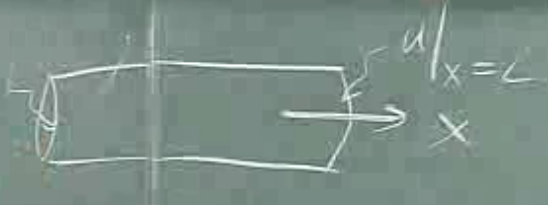
\includegraphics[height=2cm]{1_04.png}

Bu denklem ustteki gibi bir borudaki isinin dagilimini, akisini gosteriyor
olsun. $u|_{x=L}$ ile gosterilen bir sinir sarti, yani $L$ uzunlugundaki
borunun en ucunda (sagindaki) olmasi sart olan isi seviyesi. Mesela bu sart
$u|_{x=L} = T_2$ olsun, ki $T_2$ bir tekil sayi, $100^o$ , $200^o$ gibi. Simdi homojenlige
ne oldu? Ana denklem homojen, ama homojenlik testini sinir sartina uyguladigimiz
zaman $0 = T_2$ gibi bir sonuc aliyoruz, ki bu absurt bir sonuc demek ki sinir
sarti homojen degil. O zaman bu problemin tamami homojen olamaz. 

Benzer sekilde borunun oteki ucu icin tanimlanan sart gayri lineer olsa

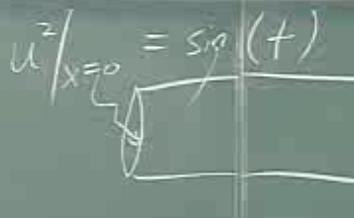
\includegraphics[height=2cm]{1_05.png}

ki bu sart o uctan bir tur sinusoidal bir enerji, isi verildigi bir durumu
tarif ediyor, o zaman ana denklem lineer olsa bile, sinir sartinda gayri
lineerlik oldugu icin problemin tamami gayri lineer olacaktir. 

Aslinda formel olarak sinir sartlarini alip 

\[ \mathcal{L}  = \frac{\partial }{\partial t} - k \partial_{xx}\]

operator tanimina bir sekilde dahil etmenin yollari var, ama biz bunlar cok
ileri seviye teknikler, bu derste bu teknikleri gormeyecegiz. 

Baslangic Sartlari

Mesela yayilma (diffusion) denklemi $u(x,t)$ icin $u(x,0) = f(x)$, yani
baslangic aninda isi dagiliminin tum boru boyunca hangi seviyelerde
oldugunun (burada bu dagilim $f(x)$) belirtilmesi , baslangic sartini
tanimlamak demektir.

Genel bir kural PDE'deki turev sayisi kadar sart tanimlanmasi
gerektigidir. Mesela iki zaman turevi var ise, iki tane kosul gerekir,
mesela $t=0$ anindaki bir kosul, arti zamana goreve turevin $t=0$ anindaki
degeri, vs. 

Soyle dusunebiliriz, $u_{xx}$'in oldugu bir denklemde $u$ elde etmek icin
iki kere entegre edilir, ve bunun sonucu olarak iki tane entegrasyon sabiti
ortaya cikar, ki bu degerler herhangi bir sayi olabilir. O iki sabiti
hesaplamak icin iki tane kosul gerekecektir. 

Genel kurali daha somutlastirirsak, ``her bagimsiz degisken icin gereken
sinir kosulu, o bagimsiz degiskenin derecesine esittir''. Tabii bu genel
bir kural, bazen gercek dunyadaki fizik problemlerinde bu gecerli
olmayabiliyor, bir problem icin duzgun sinir kosullari bulmak basli basina
bir sanat denebilir aslinda. 

Ornek

Laplace denklemi

\[ \nabla^2 u \equiv \frac{\partial ^2u}{\partial x^2} + 
\frac{\partial ^2u}{\partial y^2}  +
\frac{\partial ^2u}{\partial z^2} 
\]

ki $\nabla^2$ Laplacian operatoru olarak bilinir. 

Ustteki turden bir denklem hic kaynak akim verilmeyen sonsuz uzayda
elektrik potansiyeli alanini temsil ediyor olabilir. 

Bu denklemin bir cozumun (ki sinir sartlarina dikkat edelim) su sekilde
oldugunu gostermek kolaydir:

\[ u(\vec{x}) = \frac{1}{\sqrt{x^2+y^2+z^2}} \]

Bu Potansiyel Teori'sinde tipik bir problem, bir alan degiskeni var, ve
orijinden uzaklastikca bu degisken azaliyor, bu azalma $1 / $ uzakligin
karesi oraninda. 

Bu ``bir'' cozum, fakat bir suru 2. derece turev var ortalikta, o zaman
$x,y,z$'nin her turlu lineer fonksiyonu de aslinda bir cozumdur. Mesela

\[ u(\vec{x}) = \alpha x + \beta y + \gamma z + \delta \]

formulu de bir cozum olabilir. Niye? Herhangi bir lineer fonksiyonun iki
kere turevini alirsak o fonksiyon yokolur. 

Demek ki bu problemin tanimi eksik, sinir sartlari da tanimlanmasi gerekli,
aksi takdirde elde edilen sonuclar ozgun olmayacak. Envai turden cozum
mumkun. 

Bu problem icin tipik bir sinir kosulu $\lim_{|\vec{x}|\to \infty} u = 0$
ifadesidir. Elektrik alan ornegine donersek, elektrik alani sonsuzluga
giderken sifira dusuyor demis oluyoruz. Bir sabite gidiyor da diyebilirdik,
o da islerdi. 

O tur bir sart 

\[ u(\vec{x}) = \frac{1}{\sqrt{x^2+y^2+z^2}} \]

sonucunu saglardi, diger secenekleri elemis olurdu. Bu ornegi sinir
kosullarinin onemini belirtmek icin sectik, bu kosullar ana denklemin
kendisi kadar onemli. 

Bir nokta daha:

Soyle bir ODE dusunelim

\[ \frac{du}{dt} = 1 \]

Entegre edince genel cozum

\[ u(t) = t + c_1 \]

Fakat PDE icin

\[ u = u(x,y) \]

\[ u_x = xy \]

Burada $y$ bazli bir turev yok, basit bir PDE, cozmesi kolay, fakat
unutmayin, entegre edince

\[ u = \frac{1}{2}x^2y + [..] \]

Noktalarin oldugu yere ne gelecek? Bir sayi sabiti degil bir fonksiyon
gelecek. 

\[ u = \frac{1}{2}x^2y + g(y) \]

cunku $u$, $y$'nin bir fonksiyonu, o zaman elimize gecen $y$'nin herhangi
bir fonksiyonu olacak, ki bu fonksiyonun degeri sinir kosullari uzerinden
tanimlanmis olmali. Bunu ozellikle vurgulamak istedim cunku insanlar bu
detayi unutabiliyor.

Sinir kosulu nasil olabilir? Mesela $u(\alpha,y) = f(y)$ seklinde
olabilir. Bu kosulu yerine sokunca

\[ \frac{1}{2}\alpha^2 y + g(y) = f(y) \]

Bu bize $g(y)$'in ne oldugunu soyler

\[ g(y)  = f(y) - \frac{1}{2}\alpha^2 y \]

ve bu ornek icin nihai cozum

\[ u(x,y) = \frac{1}{2}x^2y + f - \frac{1}{2}\alpha^2 y \]

Ilginc bir ornege bakalim simdi. 

PDE'lerin ortaya cikabilecegi durumlardan biri, ayriksal parcaciklardan
olusan bir sistemin limite gittigi andir. Bu tur sartlarda ODE'lerden
olusan bir sistem limite giderken bir PDE ortaya cikartabiliyor. Sureklilik
Mekaniginden (Continuum Mechanics) bir ornek verecegiz yani.

Sistem ayriksal baslayacak, sureklilik limitine gidecek. Mesela sivilar
mekaniginde (fluid mechanics) Euler denklemi, Navier-Stokes denklemleri
sivi sisteminin (su gibi mesela) sureklilik limitidirler. Bu denklemler
sivi icindeki ufak parcaciklari tarif etmezler, sistemin butunune
bakarlar. 

Hepimiz Newton Kanunu biliyoruz (ki bu kanun bu derste ihtiyacimiz olan
yegane fizik bilgisi)

\[ m \frac{d^2x}{dt^2} = F(x) \]

Formul ne diyor? Kutle carpi ivme esittir kuvvet. Gayet basit.

Diyelim ki elimizde $N$ tane tane parcacik var, $i=1,..,N$, ve bu
parcaciklar birbirleriyle etkilesim halindeler, aralarinda bir tur cekim
var belki, ya da baska bir kuvvet. O zaman her parcacik icin ayri ayri
hareket kanunu isleyecek. Ve $i$'inci parcacik uzerinde bir kuvvet var, ve
bu kuvvet sistemdeki tum diger degiskenlerle bir sekilde bagimli. $x$ tabii
ki pozisyon degiskeni. O zaman

\[ m_i \frac{d^2x_i}{dt^2} = F_i(\vec{x}) \]

Dikkat edersek, $F$ fonksiyonuna giren parametre tum parcaciklar, yani o
parcacigin hissettigi kuvvet bir sekilde tum diger parcaciklarla alakali. 

Baslangic Sarti

$i$'inci parcacigin baslangic konumu

\[ x_i(0) = \hat{x}_i \]

Tipik olarak baslangic hizi da verilir

\[ \frac{dx_i}{dt}(0) = \hat{v}_i \]

Ustteki bir baslangic deger problemi (initial value problem). Biz bu derste
PDE bazinda sinir degerli problemlerle ugrasacagiz. 

Bu tur baslangic deger problemleri iyi huyludur, cunku, mesela bu ornekte
2. derece bir diferansiyel denklem var elimizde, ve bagimli degisken $x$
var, ve bize verilen kosulu anlamak icin alttaki resme bakalim


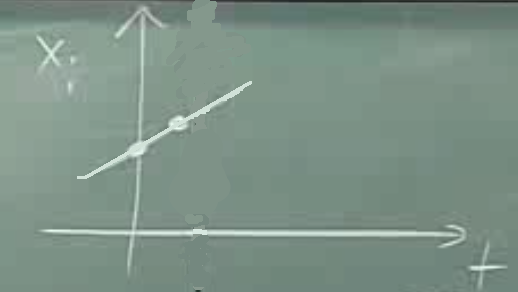
\includegraphics[height=3cm]{1_06.png}

Bize verilenler, $t=0$ aninda $x_i$ noktasinin oldugu yere ek olarak
(soldaki nokta), bir de o noktadaki egim bilgisi. Bu tur bilgi verilince,
parcacigin hangi yone gitmeye meyilli olacagini da gormus oluyoruz. Sanki
bir top ateslenmis, ve topun ates ettigi anda nerede olduguna ek olarak
topun namlusunun gosterdigi yer de bize soyleniyor.

Bu iyi huylu bir problem. Sinir degerli denklemler cok daha karmasik
olabiliyor. Bu arada ``sinir kosullu'' kelimesindeki ``sinir'' cogunlukla
bir fiziksel seye tekabul eder, mesela bir ip vardir, ve ipin ``sonunda''
yani sinirlarinda degerin ne olmasi gerektigi sabitlenir. 

Devam edelim. Kurmak istedigimiz model bir tur ``gitar teli'' modeli. 

$y_i$ = $i$'inci parcacigin yuksekligi olsun. 

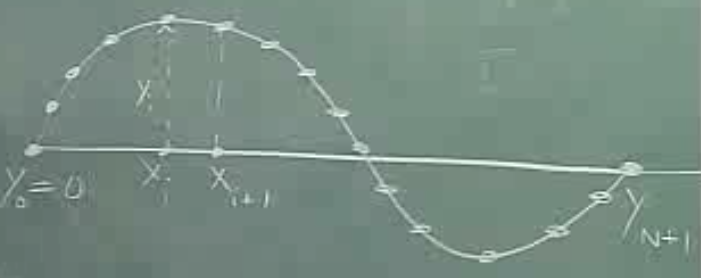
\includegraphics[height=4cm]{1_07.png}

Tel uzerinde bir suru parcacik var, tel iki ucundan sabitlenmis durumda. Bu
problemde yatay hareketle ilgilenmiyoruz, sadece yukari / asagi hareketle
ilgileniyoruz. Bir tanim daha:

\[ \Delta x = x_{i+1} - x_i  \]

Basitlestirme amaciyla bu tanimi yaptik. Tum parcaciklarin arasindaki
mesafeyi sabit, ve ayni olarak aldik. Benzer sekilde

\[ m_i \equiv m \]

Yani tum parcaciklar ayni kutleye sahip. 

Simdi Newton Kanununu parcaciklara uygulayalim [1]. 

\[ m \frac{d^2Y_i}{dt^2} = 
\tau \bigg( \frac{Y_{i+1}- Y_i}{\Delta x} \bigg) -
\tau \bigg( \frac{Y_{i}- Y_{i-1}}{\Delta x} \bigg) 
\]

Bununla ne demis olduk? $i$'inci parcacigin hissettigi cekimin, o
parcacigin saginda ve solunda bagli oldugu diger parcacikla baginin ipteki
egimi ile orantili oldugunu soylemis olduk.

$\tau$ her tel icin farkli olacak bir gerginlik sabiti, ama belli bir
telde, her parcacik icin ayni. 

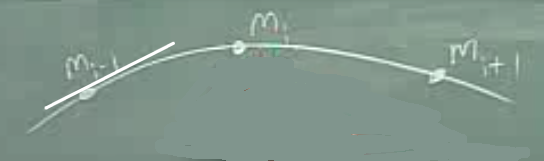
\includegraphics[height=3cm]{1_08.png}

Ustteki formul aslinda yerel turevin ``ucuz'' bir yaklasiksallamasi. 

Gerginlikle kurulan alaka akla yatkin olmali, dusunursek ipte parcacik ne
kadar yuksekte olursa uzerinde o kadar guc hissederdi, yanindaki
parcaciklar(lar) tarafindan asagi cekilirdi, ne kadar altta ise o kadar az
guc hissederdi. Tabii ``diger parcaciklara gore'' yukarida ya da asagida
olmanin olcusu de iki parcacik arasindaki ipin egimi. 

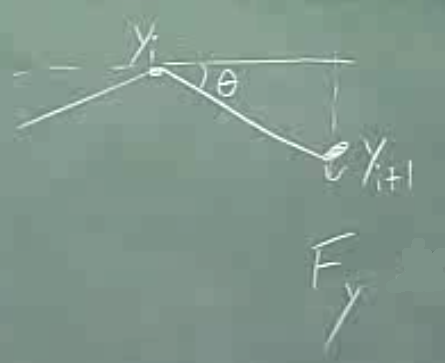
\includegraphics[height=4cm]{1_09.png}

Diger bir acidan yaklasirsak

\[ F_y \equiv \tau sin\theta \]

da diyebilirdik. Sadece sin kullandik cunku daha once belirttigimiz gibi,
sadece dikey hareketlere bakiyoruz, yatay hareketlerle ilgilenmiyoruz (o
yuzden cos yok).

Bir yaklasiksallama yapabiliriz simdi, eger $\theta << 1$ ise, yani aci 1
sayisindan cok kucuk ise, $sin\theta \approx tan\theta$ sayilabilir, bu
sonuc Taylor Serileri ile alakali ve $tan$ fonksiyonu, $sin / cos$ oldugu
icin ve sifira yakin degerlerde bolen $\theta$'nin sifira yakinligindan cos
uzerinden hep 1'e yakin olacagi icin, $tan$ bir nevi $sin$
sayilabilir. Peki bu problemde $tan\theta$ nasil hesaplanir?

\[  \tan\theta = \frac{\Delta y}{\Delta x} \]

\[ = \frac{Y_{1+1}-Y_i}{\Delta x} \]

Yani yine ayni yere gelmis olduk. 

Bu model bir ``en yakin komsu'' modelidir, her parcacik yakinindaki
parcaciktan etkileniyor. 

Ana formulu su sekilde tekrar organize ederek yazalim

\[ \frac{d^2Y_i}{dt^2} = 
\tau \frac{\Delta x}{m} \bigg[
\frac{Y_{i+1} - 2Y_i + Y_{i-1}}{\Delta x^2}
\bigg]
\]

Koseli parantez icindeki ifade Calculus'ta 2. turevin ayriksal formdaki
yaklasiksallamasi degil mi?

Ayriksal modelimiz boyle. Simdi sureklilik limitine gecmek istiyorsak,
mesela sonsuz sayida parcacik oldugu bir duruma gecmek isteyebiliriz,
$\lim_{N \to \infty}$, elimizde sonlu / belli miktarda bir tel var, bu durumda 
sonsuz sayida parcacik demek bu parcaciklarin arasindaki mesafenin sifira 
gitmesi demektir, o zaman $\lim_{\Delta x \to \infty}$. 

Formul icin bunun anlami nedir? $\Delta x$ ve $m$ arasindaki oran sonlu
(finite) bir sayiya yaklasacak demektir, ki bu sayiya yogunluk
diyebiliriz. Oran niye sifira gitmiyor? Sureklilik sistemlerin kullanilan
bir numara bu,

\[ \rho = \lim_{\Delta x \to 0} \frac{m}{\Delta x} \]

$\Delta x$'in asagi indigini dusunuyoruz, ama olabilecek cok ufak bir hacim
hayal ederek mesela molekul boyutundan daha fazla asagi inmeyecegini
soyluyoruz, $m$ ayni sekilde kuculuyor, ve oran bize bir yogunluk hesabi
veriyor.

Taylor Serileri hakkinda hizli bir ders

\[ Y_{i+1}=Y(x_i + \Delta x) \]

Eger $\Delta x$ cok kucuk ise

\[ = 
\underbrace{Y(x_i)}_{Y_i} + \Delta x \frac{dY}{dx}|_{x_i} + 
\frac{\Delta x^2}{2}\frac{dY^2}{dx^2}|_{x_i} + 
O(\Delta x^3)
\]

Daha kisa bir sekilde yazalim

\[ Y_{i+1} = Y_i + \Delta x Y_i' + \frac{\Delta x^2}{2}Y_i'' + ... 
\]

Ayni seyi $Y_{i-1}$ icin yapabiliriz

\[ Y_{i-1} = Y_i - \Delta x Y_i' + \frac{\Delta x^2}{2}Y_i'' + ... 
\]

Not: Esitligin sagindaki eksi, arti isaretlerinin nereden geldigini merak
ediyorsak, Hesapsal Bilim 1 Ders 2 notlarinda $u(x-h)$ acilimina
bakabiliriz.

Son iki formulu toplarsak

\[ Y_{i+1} + Y_{i-1} = 2Y_i + \Delta x^2 Y_i''  + O(\Delta x^4)\]

O zaman 2. turevin $x_i$'daki yaklasiksallamasi 

\[ Y_i'' = \frac{Y_{i+1} - 2Y_i + Y_{i-1}}{\Delta x^2} + O(\Delta x^2) \]

O zaman ana formulde

\[ \frac{d^2Y_i}{dt^2} = 
\tau \frac{\Delta x}{m} \bigg[\underbrace{
\frac{Y_{i+1} - 2Y_i + Y_{i-1}}{\Delta x^2}
}_{\to \frac{\partial ^2y}{\partial x^2}}
\bigg]
\]

Yani $\Delta x \to 0$ iken koseli parantez ici $\partial ^2y/\partial
x^2$'e gider. Niye kismi tureve gider? Cunku ayriksal degisimi sadece $x$
uzerinde yaptik, fakat $Y$ icinde ayni zamanda $t$ de var. Notasyon olarak
ODE dili kullanmamiz kafa karistirmasin, goruntu basit olsun diye bunu
yaptik. Ama degisimin $x$ te olmasi sebebiyle turev kismi turev oldu. 

O zaman bu sistemin sureklilik limiti, $\Delta x \to 0$ iken

\[ 
\frac{\partial ^2Y}{\partial x^2} = 
\frac{\tau}{\rho}\frac{\partial ^2y}{\partial x^2}
 \]

olacaktir. Bu denklem fizikte iyi bilinen dalga denklemidir. Insanlar
cogunlukla 

\[ c^2 = \frac{\tau}{\rho} \]

seklinde yazarlar ve $c$ boylece ``dalga hizi'' olarak kullanilabilir. 

Eger teli bir noktasinda titrettigimiz dusunursek, ve telin sonlu degil
sonsuz oldugunu dusunelim, o zaman ``hareket eden dalgalar (traveling
waves)'' fenomenini goruruz. Alttaki resimde $t=0$ aninda bir tepe noktasi
var (tele vurduk), ve ikinci resimde iki tane tepe noktasi saga ve sola
esit sekilde hareket ediyorlar. 

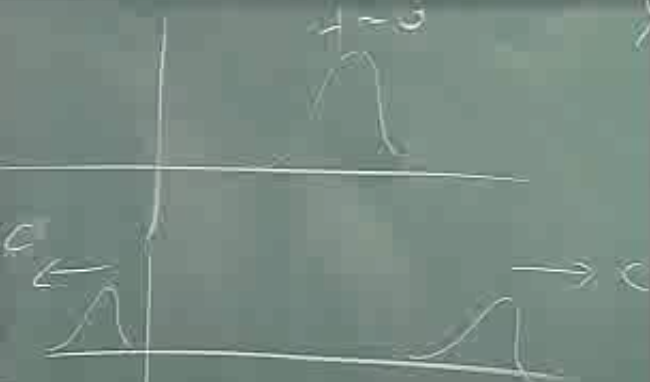
\includegraphics[height=3cm]{1_10.png}

PDE'ler ayriksal sistemlerin, ODE'lerin, sureklilik limitinde dogal olarak
ortaya cikarlar. Bu tur yaklasiksallamalari ben arastirmalarimda surekli
kullaniyorum [hoca uygulamali matematikci], akiskanlik mekaniginde mesela,
bir sivinin, molekulun kisimlarini aliyoruz, ve kisimlar birbirleri ile
etkilesimde oluyorlar. Ya da mesela yogunluk degiskenini, kutleyi bir
surekli fonksiyon haline getiririz, ve parcacik hizi yerine sivinin
tamaminin hizina bakariz. Yani bu cok kullanilan bir teknik. Cogunlukla
ayriksal bir ag yapisi icin analitik bir denklem bulmak cok zordur, o
sebeple sureklilik yaklasiksallamasi kullanilir zaten. Belki ustteki
problem icin alternatif cok kotu olmayabilirdi, mesela burada ODE'leri
matris formunda yazarak ta cozume gidebilirdik, bu cok zor olmazdi, fakat
cogu zaman bunu yapmak hakikaten zor olabiliyor.

Niye sistemi analitik olarak gormek istiyoruz? Cunku o zaman formulasyonu
istedigimiz gibi manipule ederek, analitik sekilde istedigimiz yoldan
ilerleyebiliyoruz.

* * *

Bir PDE kategorisinden bahsedelim, bu tur PDE'ler en cok kullandigim
PDE'lerden, lineer 1. derece denklemler. Ve bu arada ``karakteristikler''
kavramindan bahsedecegiz. 

1. Derece, Lineer PDE, 2 Bagimsiz Degisken

\[ u = u(x,y) \]

PDE

\[ a(x,y)u_x + b(x,y)u_y + c(x,y)u = f(x,y) \]

Operator olarak 

\[ \mathcal{L}u = f \]

\[ \mathcal{L} = a \frac{\partial }{\partial x} +
b \frac{\partial }{\partial y} +
c \frac{\partial }{\partial z} 
\]

Karakteristik kavramindan birazdan istifade edecegiz, ama simdi bu tur
denklemleri kaba kuvvet kullanarak, ``degisken degistirme (change of
variables)'' yontemi ile nasil cozulebilecegini gosterelim. 

Tanim

Cauchy Problemi: $u(\vec{x})$ tanimi gerektirir. Bu tur problemler
1. derece, 2 degisken, vs. gibi tanimlarla sinirli degil aslinda, cok daha
genel bir tanim onlar, bu tur problemlerde bir ``Caucy Verisi (Cauchy
Data)''nden bahsedilir.

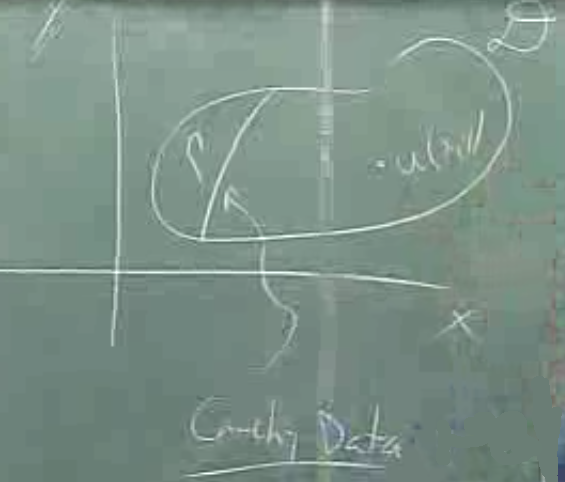
\includegraphics[height=4cm]{1_11.png}

Ustteki resimde bu veri $D$ alani (domain) icindeki $\Gamma$ ile isaretli
cizgidir, ki $u$'nun bu cizgi uzerindeki degeri diyelim ki

\[ u|_{\Gamma} = \alpha(x,y) \]

ki $\alpha(x,y)$ herhangi bir sonuc. 

Mesela $\Gamma$ cizgisi $x=sin(y)$ ile tanimli egri, ve $u$ onun uzerinde
$u=y^2$ olmali.

Bu tur bir kosula Cauch Verisi ismi veriliyor, bizim ornegimizde bu bir tur
sinir kosulunu andiriyor. 

Bir kordinat sistemi nedir? 

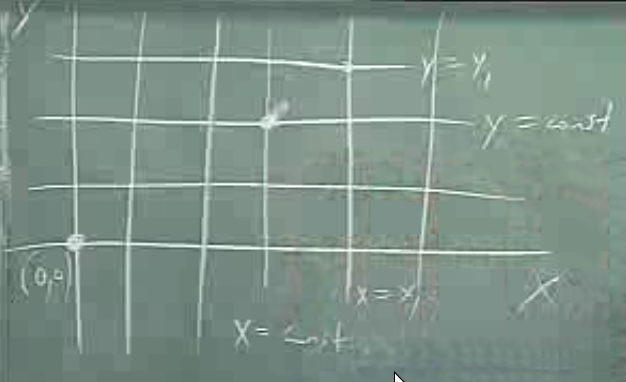
\includegraphics[height=4cm]{1_12.png}

Diyelim ki oyle bir fonksiyon kumesi var ki, onlar uzerinden PDE'lerimizi
degisik bir kordinat sisteminde temsil etmemiz mumkun olacak. 

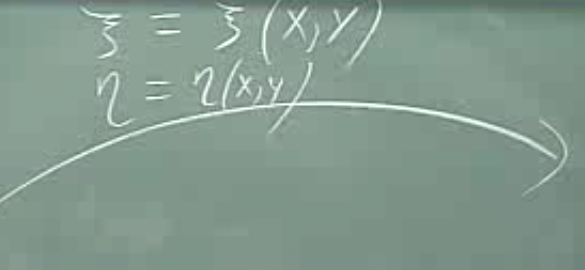
\includegraphics[height=2cm]{1_13.png}

$\xi$ ve $\eta$'yi kesit egrileri (level curves) uzerinden incelemek
mumkundur. Bu fonksiyonlari belli sabitlere esitleyip, durumlarina
bakabiliriz, sonra sabitleri degistiririz, bir daha bakariz, vs. 

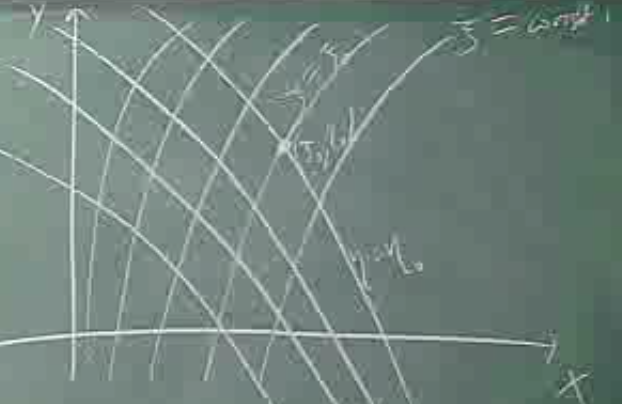
\includegraphics[height=6cm]{1_14.png}

Ustteki resimde mesela, saga yatik tum egriler, her biri degisik bir sabite
(Ingilizce const diye yazilmis) esit olacak sekildeki $\xi$ egrileri
olabilir. Sola yatik $\eta$ cizgileri de olabilir. Ortadaki nokta iki
onceki resimdeki bir noktanin bu yeni kordinata eslenmis bir nokta mesela.

Gerekliliklerimiz

Esleme, transformasyon bire bir (one-to-one) olmali. Ilk kordinat
sistemindeki her nokta, diger kordinat sistemindeki tek bir noktaya
esleniyor olmali. 

Jacobian'i yokolmayan (non-vanishing) olmali. 

\[ 
\left(\begin{array}{rr}
\xi & \eta \\
x & y
\end{array}\right) = 
\left|\begin{array}{rr}
\xi_x & \xi_y \\
\eta_x & \eta_y
\end{array}\right| =
\xi_x \eta_y - \xi_y \eta_x \ne 0
 \]

Ustteki ifade Calculus'un Dolayli Fonksiyon Teorisi (Implicit Function
Theorem of Calculus) ile alakali. Bu teorinin yerel baglamda niye birebir
esleme yarattigini merak ediyorsaniz Calculus kaynaklarina
danisabilirsiniz. 

Amac: Sunu 

\[ au_x + bu_y + cu = f \]

transform et ve suna cevir

\[ W_\xi + h(\xi, \eta)W = R(\xi,\eta)\]


\[ W(\xi,\eta) \equiv u \bigg( x(\xi,\eta),y(\xi,\eta) \bigg) \]

Birebir transformasyon istemistik, o zaman esleme geriye cevirilebilir
(invertible) de olmali, yani istersek $x,y$ degiskenlerini $\xi,\eta$
cercevesinde temsil edebiliyor olmamiz lazim. 

Dikkat: $W_\eta$ yoktur, bu sayede iki ustteki formul 1. derece ODE haline
gelir, entegre edici faktor kullanip entegre edip Cauchy Verisini
uygulayarak bu problemi cozebilirsiniz. Analitik olarak biraz karmasikliga
sebep verebilir, ama bu en azindan mumkun bir stratejidir. 

Simdi sira transformasyonu bulmaya geldi. $x,y$ degiskenlerini $\xi,\eta$
cercevesinde temsil edelim. Zincirleme Kanununu kullanalim. 

\[ \frac{\partial }{\partial x}u \equiv
\frac{\partial }{\partial x}W(\xi(x,y),\eta(x,y)) =
W_\xi\eta_x + W_\eta\eta_x 
 \]

\[ \frac{\partial }{\partial y}u =
W_\xi\eta_y + W_\eta\eta_y
 \]

Bunu orijinal denkleme sokalim

\[ 
a(\xi,\eta) \bigg[W_\xi \eta_x + W_\eta\eta_x \bigg] +
b(\xi,\eta) \bigg[W_\xi \eta_y + W_\eta\eta_y  \bigg] + 
c(\xi,\eta)W = f(\xi,\eta)
 \]

Tekrar duzenleyelim

\[ = 
\bigg[ a\xi_x + b\xi_y \bigg] W_\xi + 
\bigg[ a\eta_x + b\eta_y \bigg] W_\eta +
cW = f
 \]

Soyle sec

1.

\[ a \eta_x + b \eta_y = 0 \]

\[ \Rightarrow \frac{\eta_x}{\eta_y} = -\frac{b(x,y)}{a(x,y)}\]

2. 

\[ \xi = x \]

Boylece 

\[ h = \frac{c}{a} \]

\[ R = \frac{f}{a} \]

elde edilir. 

Unutmayalim Jacobian sartini tatmin etmemiz lazim. 

Farz edelim 

\[ \eta_y \ne 0 \]

Bu ise yarar

\[ J = \xi_x\eta_y - \cancelto{0}{\xi_y}\eta_y \]

\[ J = \eta_y \ne 0 \]

Bir dahaki derste $\eta$'yi nasil hesaplayacagimizi gorecegiz. 

---

[1] Diger bir acidan bakarsak, mesela matematikci David Mumford
turetirken ($i$ yerine $k$ kullanmis)

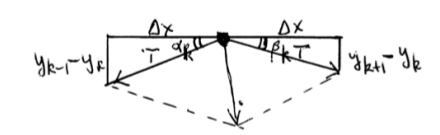
\includegraphics[height=3cm]{1_15.png}

\[ 
\tau \bigg( \frac{Y_{i+1}- Y_i}{\Delta x} \bigg) +
\tau \bigg( \frac{Y_{i-1}- Y_{i}}{\Delta x} \bigg) 
\]

kullanmis. Yani bir parcacigin uzerindeki kuvvet sagindaki ve solundaki
kuvvetlerin ``toplami'' olarak goruluyor, bu formul de ayni kapiya cikiyor.


PDE - Isi Denklemini Turetmek - Ders 2

Denklem soyle idi

\[ a(x,y)u_x + b(x,y)u_y + c(x,y)u = f(x,y) \]

Bu denklem homojen degil, cunku denklemin sol tarafi $f \ne 0$, homojenlik
icin nihai test tabii ki $u=0$ koyunca $0=0$ cikip cikmayacagi.

Cozum icin kullandigimiz fikir neydi? Kordinat sistemini transform etmek,
ki 

$\bigg(x,y\bigg) \to \bigg(\xi(x,y), \eta(x,y)\bigg)$

olsun. Bu degisimi yaparken oyle bir degisim ariyoruz ki boylece transform
edilmis PDE'miz cozulmesi kolay bir hale gelsin. 

Amac

Denklemi sadece tek bir bagimsiz degiskene gore turevi icerecek sekilde
yazmak 

\[ w_\xi + h(\xi,\eta)w  = R(\xi,\eta) \]

\[ w \equiv u \bigg( x(\xi,\eta),y(\xi,\eta) \bigg)  \]

\[ 
J = 
\left|\begin{array}{rr}
\xi_x & \xi_y \\
\eta_x & \eta_y
\end{array}\right| =
\xi_x \eta_y - \xi_y \eta_x \ne 0
 \]

Turev Transformasyonu

\[ \frac{\partial }{\partial x} = 
\frac{\partial \xi}{\partial x}  \partial_\xi + 
\frac{\partial \eta}{\partial x}\partial_\eta
\]

\[ \frac{\partial }{\partial y} = 
\frac{\partial \xi}{\partial y}  \partial_\xi + 
\frac{\partial \eta}{\partial y}\partial_\eta
\]

Bunu yapinca PDE su hale gelecek

\[ a \bigg[ a\xi_x + b\xi_y \bigg]w_\xi + 
a \bigg[ a\eta_x + b\eta_y \bigg]w_\eta + 
cw = f
 \]

Simdi $\eta$ kordinatini oyle bir sekilde secmek istiyoruz ki ustteki sag
koseli parantez icindeki terimler yokolsun. Boylece PDE'yi $\xi$ bir ODE'ye
indirgemis oluruz. Bunu elde edince entegrasyon kolaylca yapilabilir. 

\[ a \eta_x + b\eta_y = 0 \]

\[=> \frac{\eta_x}{\eta_y} = - \frac{b(x,y)}{a(x,y)} \]


Yani ikinci kordinat sistemi her ne ise, onun ortaya cikardigi kismi
turevlerinin birbirine orani katsayi fonksiyonlarinin oraninin negativine
esit.  

[burada kesildi]



\end{document}
